\documentclass[draft]{beamer}

\usepackage{fontspec}
\usepackage{hyperref}

\usepackage{xcolor}
%\usepackage{listings}
%\usepackage{courier}
%\lstset{
%basicstyle=\tiny\ttfamily, % Standardschrift
%numbers=left, % Ort der Zeilennummern
%tabsize=4, % Groesse von Tabs
%}
%\lstloadlanguages{C++}
%\DeclareCaptionFont{blue}{\color{blue}}
 
%\captionsetup[lstlisting]{singlelinecheck=false, labelfont={blue}, textfont={blue}}
%\usepackage{caption}
%\DeclareCaptionFont{white}{\color{white}}
%\DeclareCaptionFormat{listing}{\colorbox{8}{\parbox{\textwidth}{\hspace{15pt}#1#2#3}}}
%\captionsetup[lstlisting]{format=listing,labelfont=white,textfont=white, singlelinecheck=false, margin=0pt, font={bf,footnotesize}}

%\usepackage[utf8x]{inputenc}
%\usepackage{ngerman}
\usepackage{graphicx}
\usepackage{svg}




\title{Gebietserkennung}
\author{Verena Treitz, Stephan Hilb}
\date{\today}

\usepackage{beamerthemesplit}

\begin{document}

\begin{frame}
	\titlepage
\end{frame}

\section{Einführung}

\subsection{Aufgabenstellung}

\begin{frame}
	\frametitle{Die Aufgabenstellung}
	\begin{minipage}{0.60\textwidth}
		\begin{figure}
			\centering
			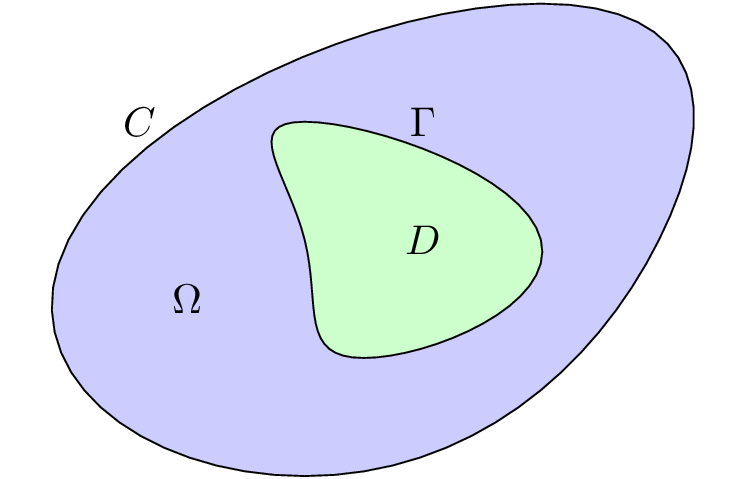
\includegraphics[width=\textwidth]{tikz/basic.png}
		\end{figure}
	\end{minipage}
	\hfill
	\begin{minipage}{0.38\textwidth}
		\begin{itemize}
			\item \pause
				homogenes Gebiet $\Omega$
			\item
				unbekannte inner Inhomogenität $D$
			\item
				Rekonstruktion des Randes $\Gamma$ von $D$
			\item \pause
				Messdaten nur auf äußerem Rand $C$
				\begin{itemize}
					\item
						angelegte Spannung $f$
					\item
						gemessener Strom $g$
				\end{itemize}
		\end{itemize}
	\end{minipage}
\end{frame}

\begin{frame}
	\frametitle{Mathematische Formulierung}
	\begin{minipage}{0.50\textwidth}
		\begin{figure}
			\centering
			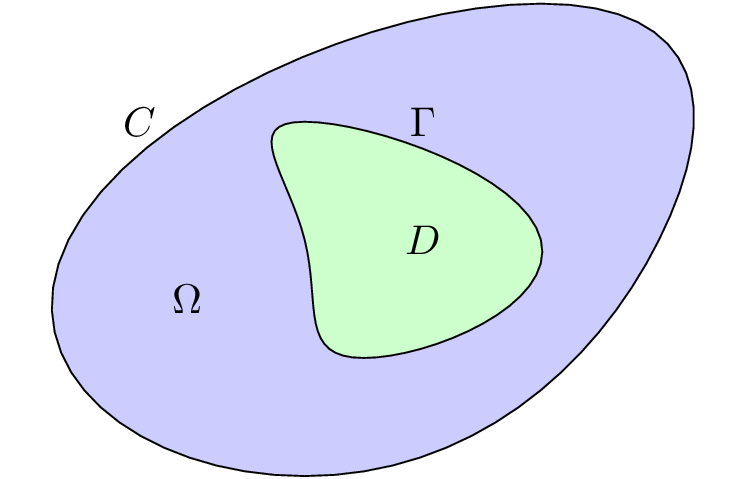
\includegraphics[width=\textwidth]{tikz/basic.png}
		\end{figure}
	\end{minipage}
	\hfill
	\begin{minipage}{0.48\textwidth}
		\pause
		\begin{align*}
			\Delta u &= 0 \quad \text{auf $\Omega \setminus D$} \\
			u|_\Gamma &= 0 \\
			u|_C &= f \\
			\tfrac{\partial u}{\partial \nu}|_C &= g
		\end{align*}
	\end{minipage}
\end{frame}

\begin{frame}
	\frametitle{Das Randwertproblem}
	\[
		\Delta u = 0 \quad \text{auf $\Omega \setminus D$}
	\]
	\begin{itemize}
		\item
			Dirichlet-Bedingungen: $u|_\Gamma, u|_C$
		\item
			Neumann-Bedingungen: $\frac{\partial u}{\partial \nu}|_\Gamma, \frac{\partial u}{\partial \nu}|_C$
		\item
			Lösbar, falls auf $\Gamma$ und $C$ jeweils eine Bedingung gegeben ist
	\end{itemize}
\end{frame}

\begin{frame}
	\frametitle{Das Inverse Problem}
	\begin{minipage}{0.5\textwidth}
		\begin{align*}
			\Delta u &= 0 \quad \text{auf $\Omega \setminus D$} \\
			u|_\Gamma &= 0 \\
			u|_C &= f \\
			\tfrac{\partial u}{\partial \nu}|_C &= g
		\end{align*}
		\pause
		Welches $\Gamma$ erfüllt dies?
	\end{minipage}
	\begin{minipage}{0.48\textwidth}
		\pause
		Ansatz:
		\begin{itemize}
			\item
				Nutze Vorwärtsproblem
			\item
				Löse $f = F(\Gamma)$
		\end{itemize}
	\end{minipage}
\end{frame}

\begin{frame}
	\frametitle{Das Vorwärtsproblem $F(\Gamma)$}
	\begin{minipage}{0.5\textwidth}
		\begin{align*}
			\Delta u &= 0 \quad \text{auf $\Omega \setminus D$} \\
			u|_\Gamma &= 0 \\
			\tfrac{\partial u}{\partial \nu}|_C &= g \\
			\implies u|_C &= f =: F(\Gamma) \\
		\end{align*}
	\end{minipage}
	\begin{minipage}{0.48\textwidth}
		\begin{itemize}
			\item \pause
				Jede Auswertung löst ein RWP $\implies$ teuer
			\item \pause
				Was ist mit $F'(\Gamma)$?
		\end{itemize}
	\end{minipage}
\end{frame}

\begin{frame}
	\frametitle{Das Vorwärtsproblem $F'(\Gamma) \cdot h$}
	\begin{minipage}{0.5\textwidth}
		\begin{align*}
			\Delta w &= 0 \quad \text{auf $\Omega \setminus D$} \\
			w|_\Gamma &= \tfrac{\partial u}{\partial \nu} h_\nu \\
			\tfrac{\partial w}{\partial \nu}|_C &= 0 \\
			\implies w|_C &=: F'(\Gamma) \cdot h \\
		\end{align*}
	\end{minipage}
	\begin{minipage}{0.48\textwidth}
		\begin{itemize}
			\item \pause
				Jacobi-Matrix berechenbar
			\item \pause
				Jede Auswertung $F'(\Gamma)\cdot h$ löst ein RWP
			\item
				Auch teuer, aber besser als FDs
		\end{itemize}
	\end{minipage}
\end{frame}

\section{Algorithmen}

\begin{frame}
	\frametitle{Diskretisierung}
	\begin{itemize}
		\item \pause
			Kurven, z.B. $C, \Gamma$:
			\begin{itemize}
				\item
					kartesisch: $n\times 2$-Matrix, $[x,y]$,
				\item
					oder äquidistant radial: $n$-Vektor
				\item
					Comsol: \texttt{InterpolationCurve}
			\end{itemize}
		\item \pause
			Dirichlet-/Neumann Randdaten
			\begin{itemize}
				\item
					kartesisch: $n\times 3$-Matrix, $[x,y,f(x,y)]$,
				\item
					Comsol: \texttt{Function Interpolation}
			\end{itemize}
	\end{itemize}
\end{frame}

\begin{frame}
	\frametitle{Algorithmen}
	Löse $H(x) := F(x) - f = 0$ durch Minimierung der Fehlerquadrate
	\begin{itemize}
		\item
			Gauß-Newton mit berechneter Jacobimatrix
		\item
			Levenberg-Marquardt (\texttt{fsolve}) mit finiten Differenzen
		\item
			Levenberg-Marquardt (\texttt{fsolve}) mit berechneter Jacobimatrix
	\end{itemize}
\end{frame}

\begin{frame}
	\frametitle{Gauss-Newton}
	\begin{itemize}
		\item
			Minimiere
			\[
				\|H(x)\|^2 \approx \|H(x_k) + H'(x_k)(x-x_k)\|^2
			\]
		\item
			$x_{k+1} := x_k - \Big(H'(x_k)^T H'(x_k)\Big)^{-1} H'(x_k)^T H(x_k)$
	\end{itemize}
\end{frame}

\begin{frame}
	\frametitle{Levenberg-Marquardt}
	\begin{itemize}
		\item
			Minimiere die Summe
			\[
				\|H(x_k) + H'(x_k)(x-x_k)\|^2 + \mu \|x-x_k\|^2
			\]
		\item
			$x_{k+1} := x_k - \Big(H'(x_k)^T H'(x_k) + \mu I \Big)^{-1} H'(x_k)^T H(x_k)$
	\end{itemize}
\end{frame}

\section{Ergebnisse}

\begin{frame}
	\frametitle{Testumgebung}
	\begin{minipage}{0.5\textwidth}
		\begin{figure}
			\centering
			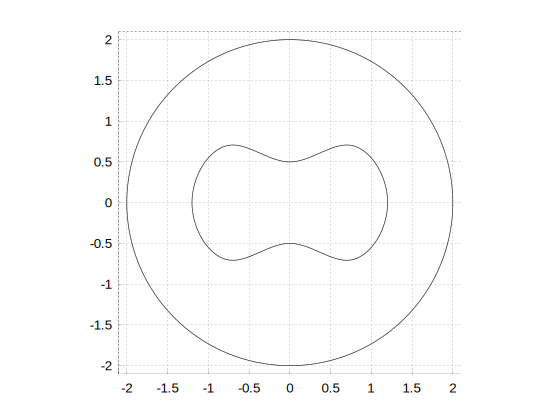
\includegraphics[width=0.8\textwidth,trim=80 0 80 0]{peanut.png}
		\end{figure}
	\end{minipage}
	\begin{minipage}{0.48\textwidth}
		\begin{itemize}
			\item \pause
				$C$: Kreis mit Radius 2
			\item
				$\Gamma$: Erdnussform, $8$ Stützstellen (radial gegeben)
			\item
				$f = 1$, $30$ Stellen, äquidistant auf $C$
			\item
				$g$ simuliert, $30$ Stellen, äquidistant auf $C$
			\item
				$\Gamma_0$: Einheitskreis
		\end{itemize}
	\end{minipage}
\end{frame}

\begin{frame}
	\frametitle{Bilder, Levenberg-Marquard FD}
	\begin{figure}
		\centering
		\includegraphics<1>[width=0.8\textwidth]{levmarq_fd_it_000.png}
		\includegraphics<2>[width=0.8\textwidth]{levmarq_fd_it_001.png}
		\includegraphics<3>[width=0.8\textwidth]{levmarq_fd_it_002.png}
		\includegraphics<4>[width=0.8\textwidth]{levmarq_fd_it_003.png}
		\includegraphics<5>[width=0.8\textwidth]{levmarq_fd_it_004.png}
		\includegraphics<6>[width=0.8\textwidth]{levmarq_fd_it_005.png}
		\includegraphics<7>[width=0.8\textwidth]{levmarq_fd_it_006.png}
		\includegraphics<8>[width=0.8\textwidth]{levmarq_fd_it_007.png}
		\includegraphics<9>[width=0.8\textwidth]{levmarq_fd_it_008.png}
		\includegraphics<10>[width=0.8\textwidth]{levmarq_fd_it_009.png}
		\includegraphics<11>[width=0.8\textwidth]{levmarq_fd_it_010.png}
		\includegraphics<12>[width=0.8\textwidth]{levmarq_fd_it_011.png}
		\includegraphics<13>[width=0.8\textwidth]{levmarq_fd_it_012.png}
	\end{figure}
\end{frame}

\begin{frame}
	\frametitle{Bilder, Levenberg-Marquard}
	\begin{figure}
		\centering
		\includegraphics<1>[width=0.8\textwidth]{levmarq_it_000.png}
		\includegraphics<2>[width=0.8\textwidth]{levmarq_it_001.png}
		\includegraphics<3>[width=0.8\textwidth]{levmarq_it_002.png}
		\includegraphics<4>[width=0.8\textwidth]{levmarq_it_003.png}
		\includegraphics<5>[width=0.8\textwidth]{levmarq_it_004.png}
		\includegraphics<6>[width=0.8\textwidth]{levmarq_it_005.png}
		\includegraphics<7>[width=0.8\textwidth]{levmarq_it_006.png}
		\includegraphics<8>[width=0.8\textwidth]{levmarq_it_007.png}
		\includegraphics<9>[width=0.8\textwidth]{levmarq_it_008.png}
		\includegraphics<10>[width=0.8\textwidth]{levmarq_it_009.png}
		\includegraphics<11>[width=0.8\textwidth]{levmarq_it_010.png}
		\includegraphics<12>[width=0.8\textwidth]{levmarq_it_011.png}
		\includegraphics<13>[width=0.8\textwidth]{levmarq_it_012.png}
	\end{figure}
\end{frame}

\begin{frame}
	\frametitle{Bilder, Gauß-Newton}
	\begin{figure}
		\centering
		\includegraphics<1>[width=0.8\textwidth]{gsnewt_it_000.png}
		\includegraphics<2>[width=0.8\textwidth]{gsnewt_it_001.png}
		\includegraphics<3>[width=0.8\textwidth]{gsnewt_it_002.png}
		\includegraphics<4>[width=0.8\textwidth]{gsnewt_it_003.png}
		\includegraphics<5>[width=0.8\textwidth]{gsnewt_it_004.png}
		\includegraphics<6>[width=0.8\textwidth]{gsnewt_it_005.png}
		\includegraphics<7>[width=0.8\textwidth]{gsnewt_it_006.png}
		\includegraphics<8>[width=0.8\textwidth]{gsnewt_it_007.png}
		\includegraphics<9>[width=0.8\textwidth]{gsnewt_it_008.png}
		\includegraphics<10>[width=0.8\textwidth]{gsnewt_it_009.png}
		\includegraphics<11>[width=0.8\textwidth]{gsnewt_it_010.png}
		\includegraphics<12>[width=0.8\textwidth]{gsnewt_it_011.png}
		\includegraphics<13>[width=0.8\textwidth]{gsnewt_it_012.png}
		\includegraphics<14>[width=0.8\textwidth]{gsnewt_it_013.png}
		\includegraphics<15>[width=0.8\textwidth]{gsnewt_it_014.png}
	\end{figure}
\end{frame}

\begin{frame}
	\frametitle{Vergleich, $\|x_k - x\|$}
	\fontsize{8pt}{10pt}\selectfont
	\begin{table}
		\centering
	\begin{tabular}{r|rrr}
 k  &    levmarqfd & levmarq  &  gsnewt \\ \hline
00  &    0.7616    & 0.7616   &  0.7616 \\
01  &    0.2544    & 0.3245   &  0.2931 \\
02  &    0.2585    & 0.3100   &  0.3291 \\
03  &    0.1603    & 0.1881   &  0.1243 \\
04  &    0.1122    & 0.1505   &  0.0897 \\
05  &    0.0664    & 0.1147   &  0.0629 \\
06  &    0.0576    & 0.0919   &  0.0517 \\
07  &    0.0544    & 0.0802   &  0.0478 \\
08  &    0.0518    & 0.0654   &  0.0451 \\
09  &    0.0500    & 0.0617   &  0.0448 \\
10  &    0.0508    & 0.0587   &  0.0442 \\
11  &    0.0418    & 0.0556   &  0.0443 \\
12  &    0.0426    & 0.0532   &  0.0441 \\
13  &              &          &  0.0442 \\
14  &              &          &  0.0441
	\end{tabular}
	\end{table}
\end{frame}

\begin{frame}
	\frametitle{Implementierung}
	\begin{itemize}
		\item
			Referenzierung von geometry-features
		\item
			Funktioneninterpolation in 2D benötigt Daten in externer Datei
		\item
			Funktioneninterpolation in 2D nur linear
		\item
			Punkte auf interpolierten Kurven generieren?
	\end{itemize}
\end{frame}

\begin{frame}
	\frametitle{Quellen}
	\begin{itemize}
		\item
	William Rundell, 2008, Recovering an obstacle and a nonlinear conductivity 	from Cauchy data ; Inverse Problems 24
\item
 F. Hettlich, W. Rundell, 1998, The determination of a discontinuity in a conductivity from a single boundary measurement ; Inverse Problems 14 67-82
 \item
	 \url{http://www.mathematik.uni-wuerzburg.de/~borzi/proj_elliptic.pdf}
 \item
 Comsol Modelle
 \item
 Skript der Vorlesung "Einführung in die Optimierung" von Prof. Dr. B. von Harrach, WS 2013/14
	\end{itemize}
\end{frame}


\end{document}
